\subsection{Compact Muon Solenoid}
\label{sec:Exp_CMS}
\subsubsection{Introduction}

CMS is a general-purpose detector designed for detecting various particles which are being produced in pp collisions at LHC. Its main feature is a huge magnet to create a magnetic field of 4T to curve charged particles in the tracking system and 2T outside to curve muons in the muon system.\\

CMS detector is a cylindrically symmetric with a colliding beam as a central axis. The detector consists, from inner to outer layer,  of a tracking system, an electromagnetic calorimeter (ECal), a hadronic calorimeter (HCal), a magnet and a muon system. Having the tracking system, ECal and HCal inside of a large solenoid makes the detector "compact". A segment of a CMS slice in $r-\phi$ plane is shown in Fig.~\ref{fig:CMS_slice}.\\

When a heavy particle is produced in a collision, it decays immediately, and we detect its long-living decay products including an electron, a photon, a muon, a neutral hadron or a charged hadron. Depending on the trace left by a particle in different subdetectors we can identify a particle. Electrons and positrons leave curved tracks in the tracking system and then induce showers in the electromagnetic calorimeter (ECal) where they are typically stopped. Photons induce the same electromagnetic showers is ECal however, as neutral particles, they do not leave tracks in the tracking system. Hadrons normally travel through the ECal undisturbed and induce a hadronic shower in the hadronic calorimeter (HCal). Charged and neutral hadrons can be distinguished from each other by checking whether they leave a track in the tracking system or not. Muons are the only particles which are not stopped by the layer of ferrum and leave tracks in the CMS muon system. Neutrinos are not detected by CMS. \\  

\begin{figure}[htb]
  \begin{center}
    {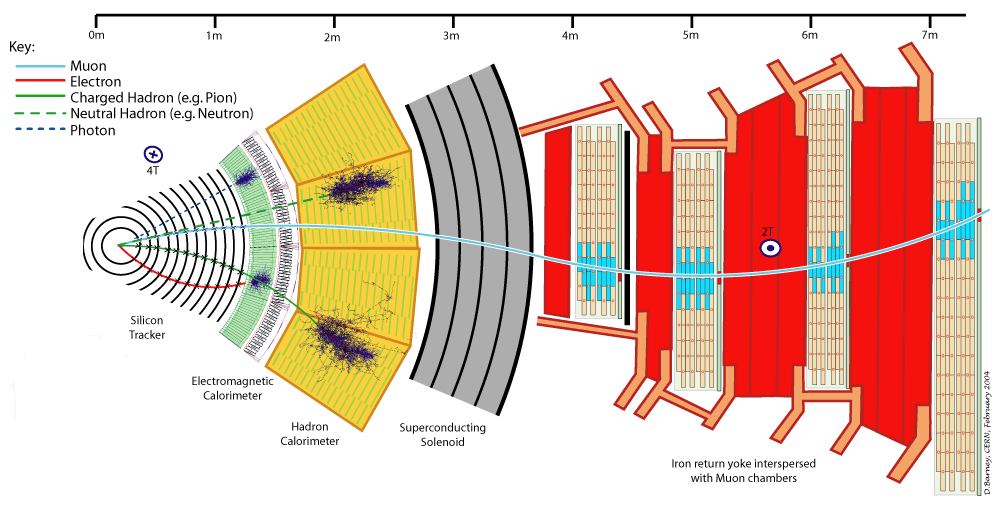
\includegraphics[width=0.98\textwidth]{../figs/Exp/CMS_Slice.png}}
    \caption{CMS slice.}
    \label{fig:CMS_slice}
  \end{center}
\end{figure}

% CMS detector geometry and variables

% In this dissertation...
In $W\gamma$ measurement we have muons and electrons as final state particles. They are both affected by CMS magnetic field allowing the tracking system and the muon system to measure their trajectory parameters and momenta.\\
In this dissertation we use the information of the primary vertex determined by the tracking system to select our events. Also the tracker provide us the information about electrons trajectories and momenta in the electron channel and distinguishes between electrons and photons.\\

\subsubsection{Magnet}

A magnetic field in a particle detector is necessary to measure momenta of charged particles by track curvatures. The higher the momentum is, the less a particles's path is affected by the magnetic field. In CMS it is done in the tracking system for all charged particles and in the muon system for muons.\\

The CMS magnet is placed between layers of HCal and a muon system. It creates a magnetic field of 4T inside the magnet, for the tracking system, and 2T outside the magnet, for the muon system. It is necessary to have stronger field in the tracking system because a density of tracks is much higher there than in the muon system and also the tracking system is much smaller and, therefore, more significant cuvature is necessary to measure the momentum with high precision.\\

The magnet is made of superconducting wires. An electric current flowing in the wires creates a uniform field inside the solenoid and also provides a magnetic filed of a certain configuration outside the solenoid.\\

\subsubsection{Tracking System}

The tracking system measures track geometry including particles trajectories and locations of primary and secondary vertices and momenta of charged particles. It needs to disturb particles as little as possible so that they can pass through. Therefore, just a few measurements must be enough to reconstruct the track. The accuracy of a measurement of each hit is 10~$\mu$m.\\

The tracking system consists of silicon pixels and silicon strips (Fig.~\ref{fig:tracker_slice}). Collision tracks start at the center and then cross the layers of the tracking system. Tracks are straight in $r-z$ plane and curved by the magnetic field in the $r-\phi$ plane. The acceptance of the tracker system in $r-z$ plane is geometrically limited by $\eta=2.5$ ($\eta=-\ln[ {\tan{\theta/2}}]$, where $\theta$ is a polar angle).\\

The pixel tracker is the closest subsystem of CMS to the collision point thus it receives the largest particle flux: at~8~cm from the collision point the flux is about~10~million $1/(cm^2 s)$, and the pixel detector with its~65~millions sensors is capable to reconsruct all these tracks. It consists of three layers of cylinders in the barrel with radii of~4~cm,~7~cm and~11~cm and four disks in the endcap, two disks at each side. The tracker is designed in such a way that a single track hits multiple sensors. Then the trajectory is reconstructed based on how much charge is collected on each sensor. This allows us to reach a spacial resolution of 15-20~$\mu$m which is much smaller than a distance between sensors.\\

The strip tracker is placed right after the pixel tracker and occupies the detector volume up to~130~cm aound the beam axis. The strip tracker consists of four parts: the tracker inner barrel (TIB), the tracker inner disks (TID), the tracker outer barrel (TOB) and the tracker endcap (TEC) as shown in Fig.~\ref{fig:tracker_slice}. In the strip tracker there are over 15,000 sensitive modules with a total number of~10~million strips. Each sensitive module consists of a set of sensors, its support structure and readout elements.\\

%electric charge and amplification

%limitations

\begin{figure}[htb]
  \begin{center}
    {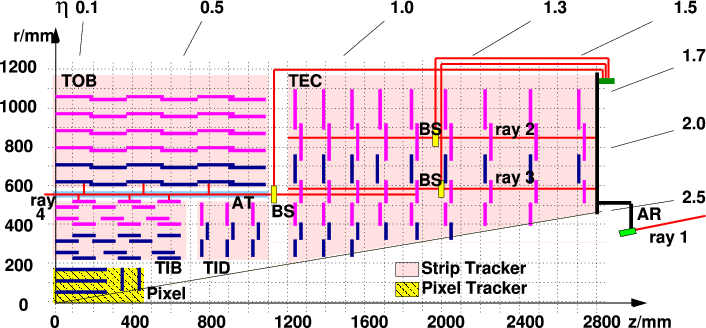
\includegraphics[width=0.8\textwidth]{../figs/Exp/tracker_slice.png}}
    \caption{Slice of the CMS tracking system in $r-z$ plane.}
    \label{fig:tracker_slice}
  \end{center}
\end{figure}

\subsubsection{Electromagnetic Calorimeter}

The ECal measures energy of electrons and photons and also measures geometries of their trajectories. Electrons and photons interact with the ECal substance by inducing electromagnetic showers. Traces left by photons and electrons in the ECal are the same. To distinguish between these two particles, it is necessary to perform matching to the track in the tracking system. If there is a track, then there is an electron (or positron). If there is no track, then the particle is a photon.\\

The Ecal is a layer between the tracking system and the HCal. It is made of high-density lead tungstate crystals arranged in a barrel section and two endcap sections. The crystals work as scintillators. When electrons and photons pass through it, it produces light proportional to the particle's energy. The scintillated light then is amplified by photomultipliers producing signals on sensitive elements.\\

It is important for the Ecal to be able to distinguish between high energetic photons and pairs of lower energetic photons e.g. from a $\pi^0$ decay. It is especially difficult in the endcap sections where angle between two photon trajectories is small. Ecal preshowers located in front of the endcaps which have much smaller granularity provide extra spacial precision. Their strips are~2~mm wide compared to~3~cm wide crystals in the main volume of the ECal.\\

%(Why muons and hadrons don't release their energy here?)
%limitations

\subsubsection{Hadron Calorimeter}

The HCal is placed right after the ECal and is the last subdetector within the magnet. The HCal measures energies of charged and neutral hadrons. In addition, the HCal determines the track parameters. Match to the tracking system has to be done: if a matching track found, then it is a chagred hadron otherwise it is a neutral hadron. \\
%(Why muons don't release their energy here? Would photons and electrons release the energy here?)

The HCal consists of alternate layers of absorbers and scintillators. Hadrons hit brass or steel plate of absorber producing secondary particles. When emerge into the scintillator, the particles induce hadronic and electromagnetic showers and emit blue-violet light which is further shifted to the green region and read out by special boxes within the HCal. The secondary hadrons produced during the interaction with the absorber interact with the next absorber producing more showers in the next layers of scintillators and also affect the total enegry deposit. All hadrons must be stopped inside the layers of the HCal.\\

%HCal Sampling calorimeter (?)
%Hybrid Photodiodes

\subsubsection{Muon System}

Muons pass through the ECal, the HCal and the magnet without interacting. They are the only particles which are registered in the muon system which is placed outside the magnet and which is the largest part of CMS detector.\\

There are four concentric layers of muon detectors (stations) and iron return yoke between them. Muons induce several hits in the muon stations which are later fitted and matched to the tracking system measurements to provide the best possible resolution in the measurements of all parameters of the muon's trajectory and momentum.\\

Overall, there are 1400 muon chambers including 250 drift tubes (DTs), 540 cathode strip chambers (CSCs) and 610 resistive plate chambers (RPCs).\\

The system of DTs measures positions of muons in the barrel. Each DT chamber is about~2~m by~2.5~m in size. It consists of~12~layers of aluminium which are groups by four. There are up to~60~drift tubes in a layer. The middle group of layers measures $z$-coordinate and two other groups determine the perpendicular coordinate.\\

Each drift tube is~4~cm in width, is filled with a gas and has a wire inside. When a charged particle passes through the volume, it ionizes atoms and the wire receives an electric charge.\\

% (how it works? why do we need it?)

% Copypaste: In total there are 1400 muon chambers: 250 drift tubes (DTs) and 540 cathode strip chambers (CSCs) track the particles’ positions and provide a trigger, while 610 resistive plate chambers (RPCs) form a redundant trigger system, which quickly decides to keep the acquired muon data or not. 

cathode strip chambers
resistive plate chambers

\begin{figure}[htb]
  \begin{center}
    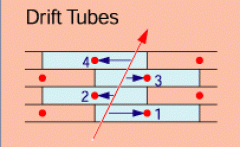
\includegraphics[height=2.5 cm]{../figs/Exp/muonSystem_driftTubes.png}\quad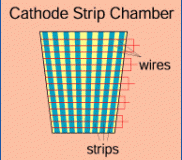
\includegraphics[height=2.5 cm]{../figs/Exp/muonSystem_CSC.png}\quad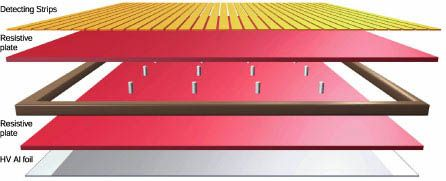
\includegraphics[height=2.5 cm]{../figs/Exp/muonSystem_RPC.png}
    \caption{Components of the CMS muon system. Left to right: drift tubes, cathode strip chambers (CSCs), resistive plate chambers (RPCs).}
    \label{fig:muonSystem}
  \end{center}
\end{figure}


\subsubsection{Triggering and Data Aquisition}
Level-I trigger
High Level Trigger

\subsubsection{Event Reconstruction}
Where to place particle reconstruction, particle flow algorithm and MET? Check other theses

Acceptance: particles which are too collinear and go to pipe; particles which get curved too strongly
